\documentclass[a4paper]{scrartcl}%{{{

\usepackage{float}
\usepackage{tikz}
\usetikzlibrary{arrows,automata}
\usepackage{pgf}
\usepackage[utf8]{inputenc} % this is needed for umlauts
\usepackage[ngerman]{babel} % this is needed for umlauts
\usepackage[T1]{fontenc}    % this is needed for correct output of umlauts in pd
\usepackage{amssymb}
\usepackage{amsmath}
\usepackage{mathabx}
\usepackage{mathrsfs}
\usepackage{dsfont}
\usepackage{graphicx}
\usepackage{fancyhdr}
\usepackage{lastpage}
\usepackage{imakeidx}
\setlength{\parskip}{\medskipamount}
\setlength{\parindent}{0pt}
\usepackage{enumitem}
\usepackage{hyperref}
\usepackage{verbatim}

%%%%%%%%%%%%%%%%%%%%%%%%
% Kopf- und Fusszeilen %
%%%%%%%%%%%%%%%%%%%%%%%%
\pagestyle{fancy}
\lhead{
        Maximilian Roth
}
\chead{Logik-Tutorat Lösungen Blatt 9\\}
\rhead{
    \begin{tabular}{rr}
        \today{} \\
        Seite \thepage{} von \pageref{LastPage}
    \end{tabular}
}
\lfoot{}
\cfoot{}
\rfoot{} 

%%%%%%%%%%%%%%%%%%%%%%%%
% Anfang des Dokuments %
%%%%%%%%%%%%%%%%%%%%%%%%%}}}

\begin{document}
\section*{Disclaimer}%{{{
\label{sec:disclaimer}
Auch in diesem Dokument können sich Fehler befinden!\\
Sie sind nicht die Musterlösung der Aufgaben, sondern selbst erstellte Lösungen.\\

Als generelle Lektüre kann ich nur das Skript von Markus Junker aus dem WS 17/18 empfehlen:\\
\url{http://home.mathematik.uni-freiburg.de/junker/skripte/InfoLogik.pdf}\\
Hier ist vieles sehr genau und verständlich erklärt.%}}}

\section*{}%{{{
\label{sec:aufgabe_1}

    \begin{figure}[H]
        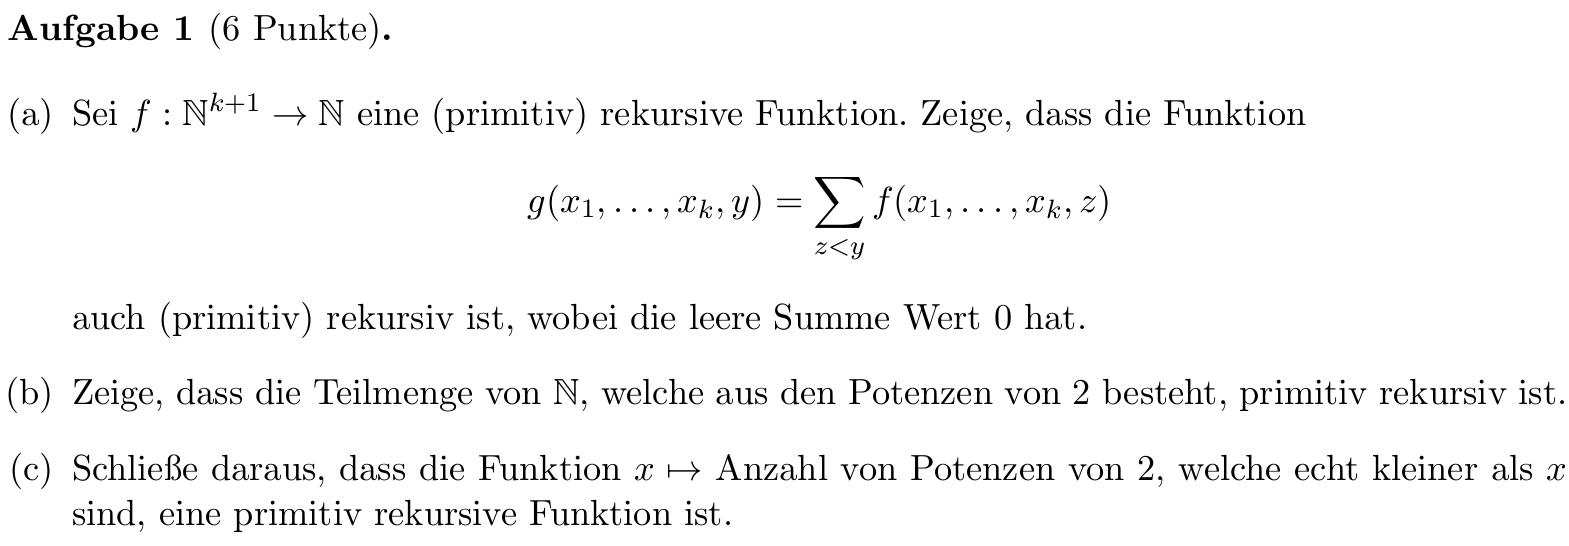
\includegraphics[scale=0.3]{./A-1.png}
        \label{fig:}
    \end{figure}

    \begin{itemize}
        \item a)\\
            $g(x_1,\dots,x_k,y) =
            \begin{cases}
                0, &\text{ falls }y = 0\\
                g(x_1,\dots,x_k, y\dotdiv 1) + f(x_1,\dots,x_k,y\dotdiv 1), &\text{ sonst }\\
            \end{cases}$ 
        \item b)\\
            Wegen Lemma 3.9 im Skript ist\\ 
            $C = \{(x,y) \in \mathds{N}^2 | \exists z < y (z \in PRIM\backslash \{2\} \land z|x)\}$ primitiv rekursiv\\
            (weil PRIM,\{2\} und $\{(z,x) \in \mathds{N}^2| 1 \leq z < x \land z|x\}$ primitiv rekursiv sind).\\
            Somit ist auch die Menge B gegeben durch die Charakteristische-Fkt:\\
            $\chi_B(x) = \chi_C(x,S(x))$ primitiv rekursiv.\\
            Man sieht, dass $ \mathds{N}\backslash B$ die Menge aller Zweierpotenzen ist.\\
            \begin{figure}[H]
                \centering
                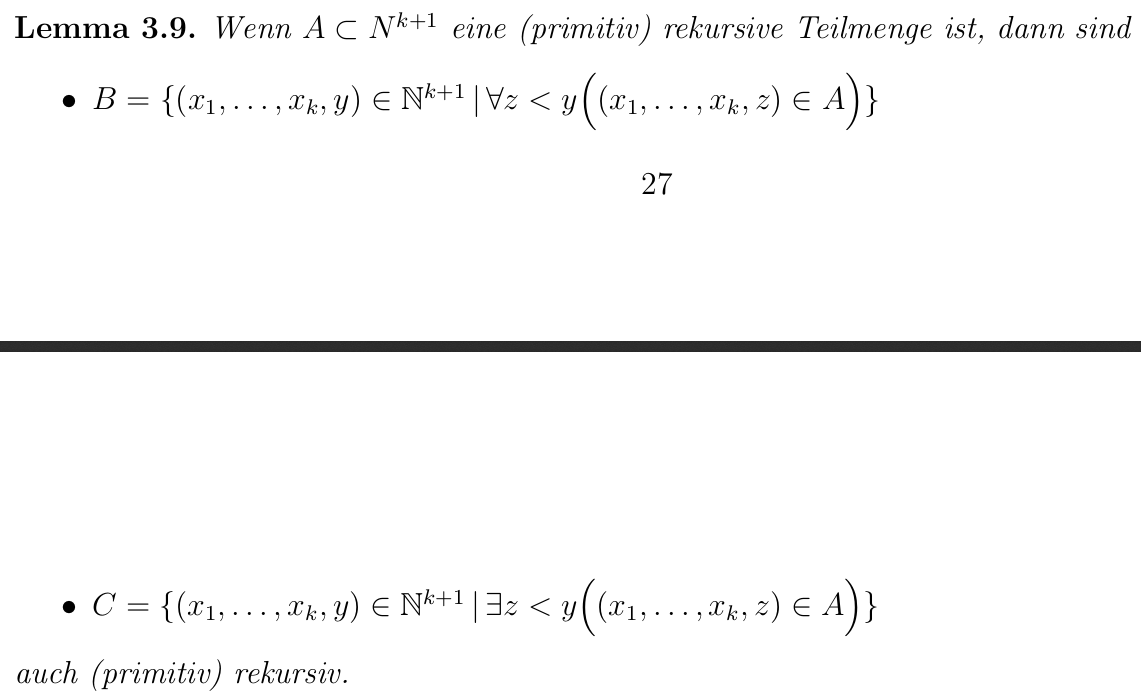
\includegraphics[scale=0.3]{./Lemma-3-9.png}
                \caption{Lemma 3.9}
                \label{fig:./Lemma-3-9}
            \end{figure}
            
        \item c)\\
            $g(x) =
            \begin{cases}
                0, &\text{ falls }x = 0\\
                g(x\dotdiv 1) + \chi_{2en}(x\dotdiv 1), &\text{ sonst }\\
            \end{cases}$\\
            Da $\chi_{2en}$ p. rek. ist ist auch g p. rek.
    \end{itemize}


%}}}

\newpage

\section*{}%
\label{sec:aufgabe_2}%{{{

    \begin{figure}[H]
        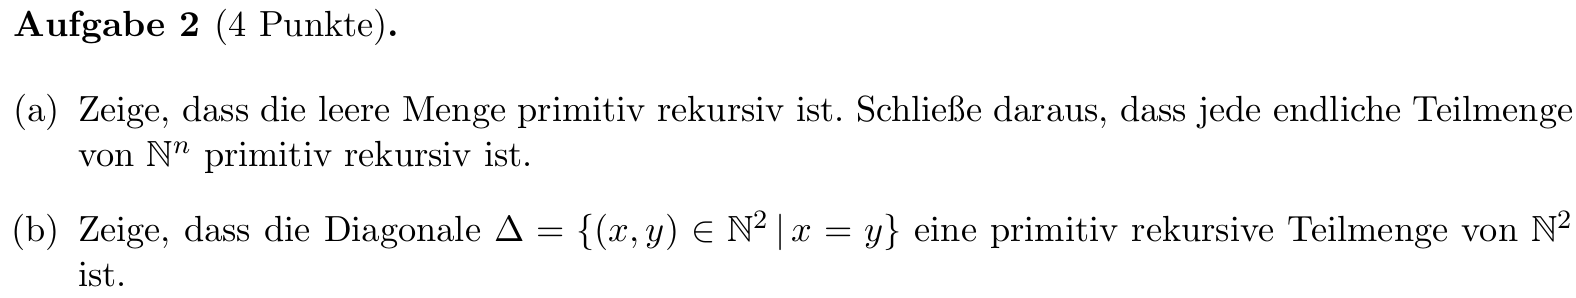
\includegraphics[scale=0.3]{./A-2.png}
        \label{fig:}
    \end{figure}

    \begin{itemize}
        \item a)\\
            Die Charakteristische-Fkt. der leeren Menge ist die konstante 0-Fkt.\\
            Diese ist bekanntermaßen p. rek.\\
            \\Mit Korollar 3.8 folgt die zweite Behauptung direkt mit A = $\emptyset$:\\
            \begin{figure}[H]
                \centering
                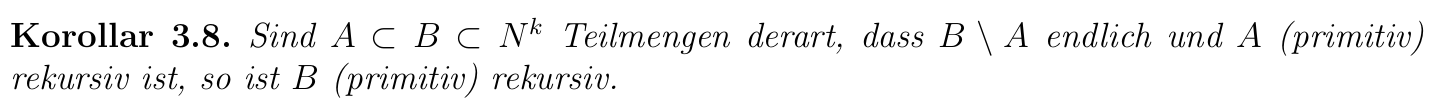
\includegraphics[scale=0.3]{./Kor-3-8.png}
                \label{fig:./Kor-3-8}
            \end{figure}
        \item b)\\
            $\chi_{\Delta}(x,y) = h(|x - y|)$\\
            Wobei für h gilt:\\
            $h(x) =
            \begin{cases}
                1, &\text{ falls }x = 0\\
                0, &\text{ sonst }\\
            \end{cases}$\\
            h und $|x-y|$ sind p. rek $\Rightarrow \Delta$ ist p. rek.\\
    \end{itemize}

%}}}

\newpage

\section*{}%{{{
\label{sec:aufgabe_3}

    \begin{figure}[H]
        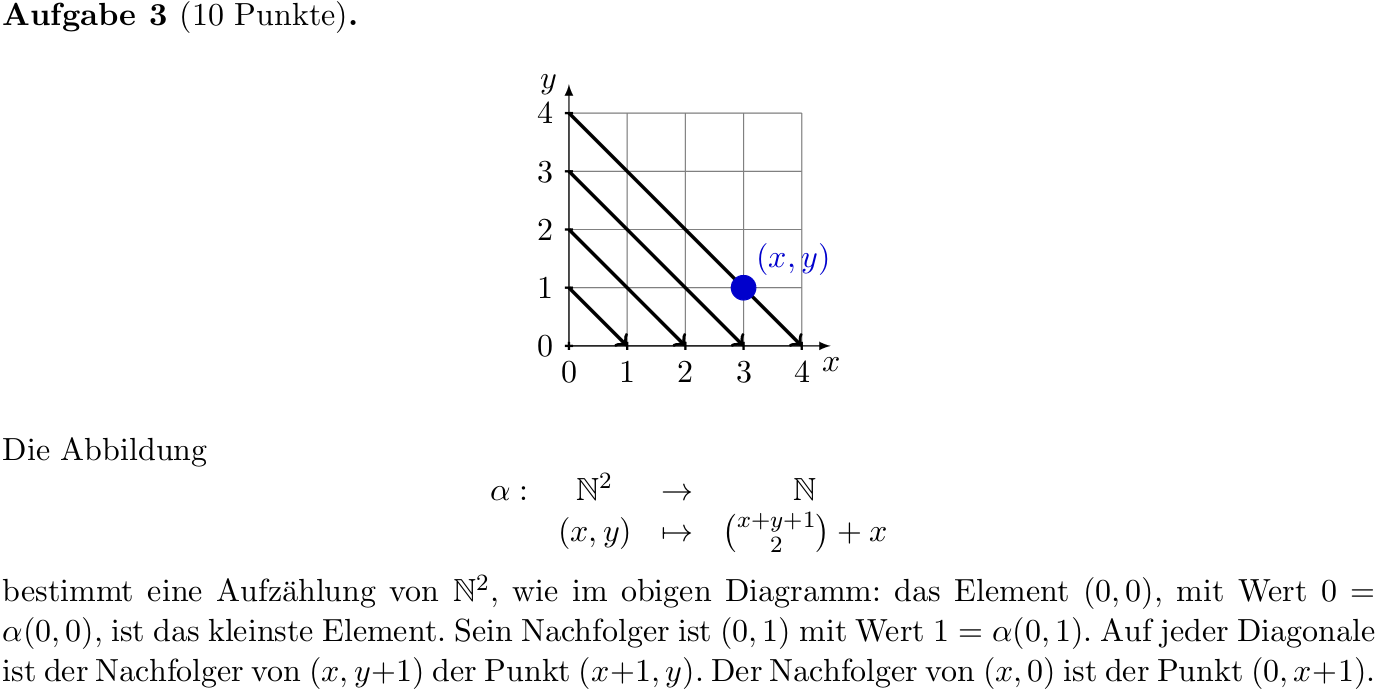
\includegraphics[scale=0.3]{./A-3.png}
        \label{fig:}
    \end{figure}

    \begin{figure}[H]
        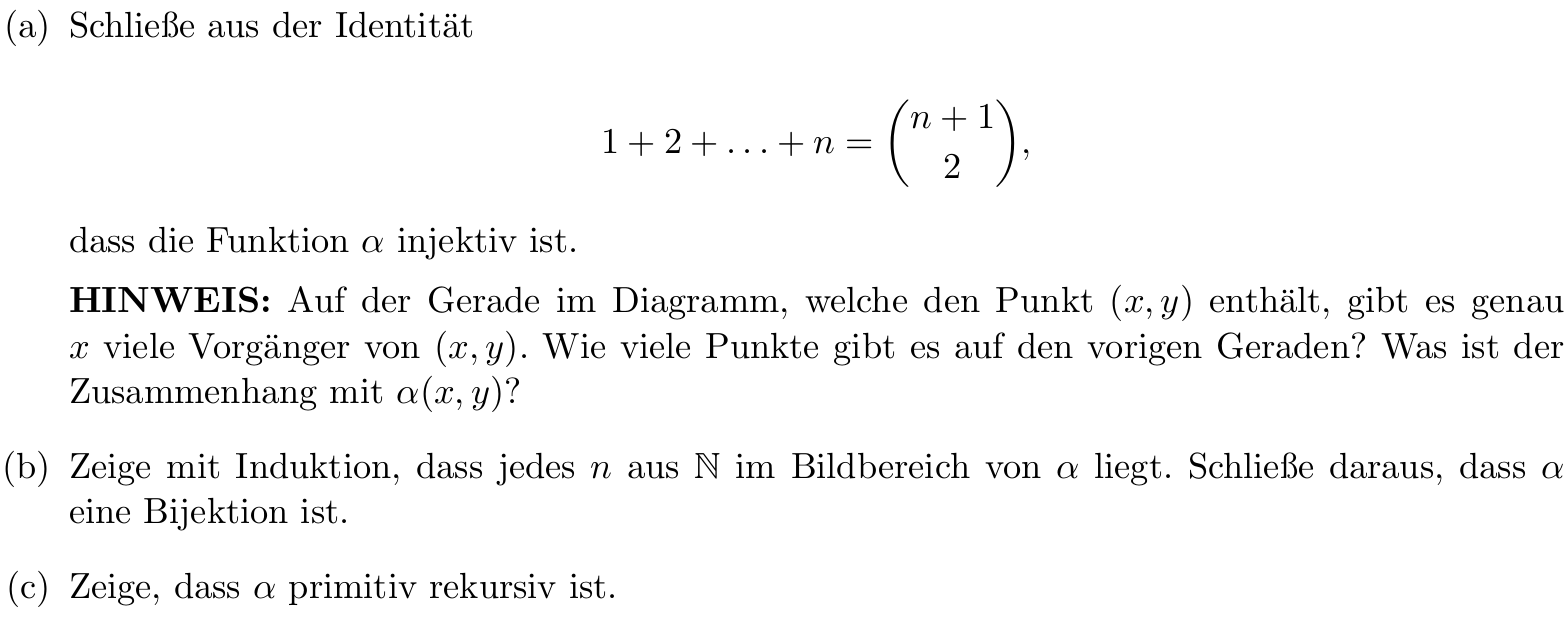
\includegraphics[scale=0.3]{./A-3-2.png}
        \label{fig:}
    \end{figure}


    \begin{itemize}
        \item a)\\
            \underline{Annahme:} Sei $\alpha(x,y) = \alpha(x',y')$, aber $x+y < x'+y'$\\
            \\$\Leftrightarrow \binom{x+y+1}{2} + x = \binom{x'+y'+1}{2} + x'$\\
            $\Leftrightarrow 1 + \dots + (x+y) + x = 1 + \dots + (x'+y') + x'$\\
            $\overset{x+y < x'+y'}{\Rightarrow} 0 = (x + y + 1) + \dots + (x' + y') + x' - x$\\
            \\Widerspruch $\Rightarrow x + y = x' + y'$\\
            \\$\Rightarrow 1+\dots+(x+y)+x = 1+\dots+(x+y)+x'$\\
            $\Leftrightarrow x = x'$\\
            $\Rightarrow y = y'$\\
        
        \item b)\\
            Wir zeigen via Induktion über $n \in \mathds{N}$\\
            \begin{itemize}
                \item IA: n = 1\\
                    $n = 1 = \alpha(0,1) = \binom{0+1+1}{2}+0 = \binom{2}{2}+0 = 1+0=1$\\
                \item IV: Gelte für ein n: $n = \alpha(j,h)$\\
                \item IS: $n \rightarrow n+1$\\
                    $n+1 = \alpha(x,y)+1$\\
                   \begin{itemize}
                        \item \underline{Fall 1:} y=0\\
                            $\overset{Hinweis}{\Rightarrow} n+1=\alpha(0,x+1)$
                        \item \underline{Fall 2:} $y \neq 0\\
                            \overset{Hinweis}{\Rightarrow} n+1=\alpha(x+1,y-1)\\
                            = \binom{x+1+y-1+1}{2}+x+1\\
                            = \binom{x+1+y}{2}+x+1\\
                            = \alpha(j,h) + 1$\\
                   \end{itemize} 
            \end{itemize}
            Aus injektiv und surjektiv folgt bijektiv.\\
        \item c)\\
            $\alpha(x,y) = g(x+y) + x = g(x+y) + \Pi^2_1(x,y)\\
            \\g(n) =
            \begin{cases}
                0, &\text{ falls }x=0\\
                g(n\dotdiv1) + n, (\text{ oder }\Pi^1_1(n)), &\text{ sonst }\\
            \end{cases}$\\
            Damit ist $\alpha$ p. rek.\\

    \begin{figure}[H]
        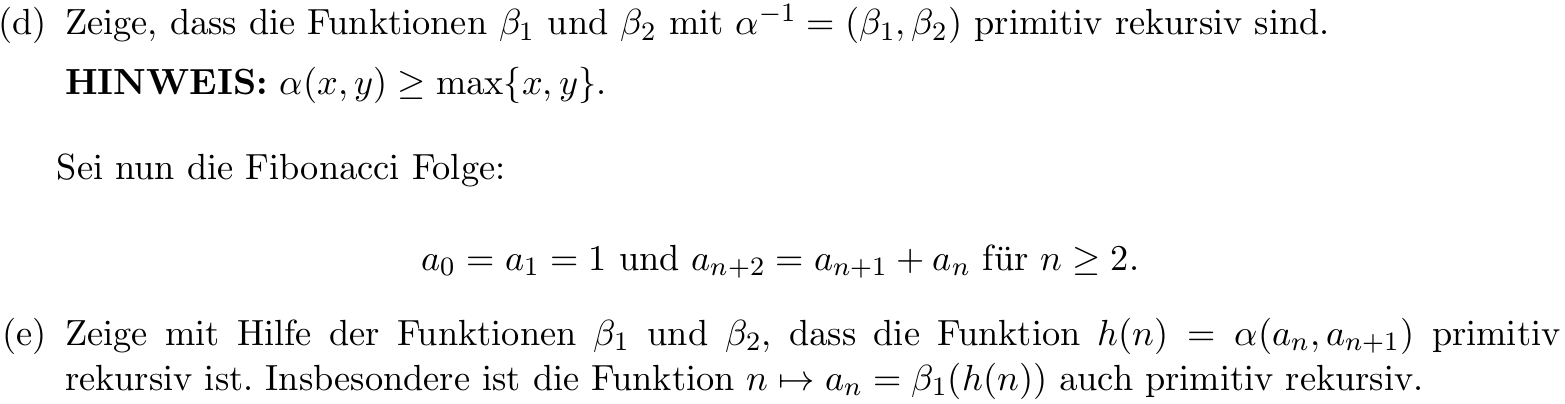
\includegraphics[scale=0.3]{./A-3-3.png}
        \label{fig:}
    \end{figure}
            
        \item d)\\
            Wir sollen zeigen, dass die Umkehrfunktion von $\alpha(x,y) = n$, also $\alpha^{-1}(n) = (\beta_1(n), \beta_2(n))$ p. rek. ist.\\
            $\alpha^{-1}$ ist offensichtlich p. rek., wenn $\beta_1 \text{ und } \beta_2$ es sind.\\
            \\Dazu suchen wir also zunächst diese beiden Funktionen und zeigen dann, dass sie p. rek. sind.\\
            \\Wir definieren zunächst d(n), die uns für eine Zahl die ursprüngliche Diagonale gibt wie folgt:\\
            $d(n) =
            \begin{cases}
                0, &\text{ falls }n=0\\
                d(z) +  (z + 2 \dotdiv \alpha(0,d(z)+1)), &\text{ falls }n=z+1\\
            \end{cases}$\\
            d(n) ist offenbar p. rek.\\
            \\Sei nun $\beta_2(n) = n \dotdiv \alpha(0, d(n))$, dann ist auch $\beta_2$ p. rek.\\
            \\Und zuletzt $\beta_1(n) = d(n) \dotdiv \beta_2(n)$ (auch klar p. rek.)\\
            $\Rightarrow \alpha^{-1}$ ist primitiv rekursiv.\\ 
        \item e)\\
            Es gilt: $h(n+1) = \alpha(a_{n+1},a_{n+2}) = \alpha(\beta_2(h(n)), \beta_1(h(n))+\beta_2(h(n)))$,\\
            Da $a_{n+1} = \beta_2(h(n))$ und\\
            $a_{n+2}=\beta_1(h(n)) + \beta_2(h(n))$ ist.\\
            \\Es gilt also:\\
            $h(n) = 
            \begin{cases}
                1, &\text{ falls }n=0\\
                \alpha(\beta_2(h(z)), \beta_1(h(z)) + \beta_2(h(z))), &\text{ falls }n=z+1\\
            \end{cases}$\\
            $\Rightarrow$ h(n) ist primitiv rekursiv.\\
    \end{itemize}
    
%}}}

\end{document}
